% =====================================================================================================
% EarthPortal: curation and FAIRness of the semantic artefacts
% Emmanuel Nyandu Kagarabi, internship at CNRS / Data Terra (1 September to 31 October 2026)
% Meeting with TIB, 13 November 2026: 10 minutes.

% Compile with pdfLaTeX (TeX Live, Overleaf):  latexmk -pdf emmanuel_dataTerra_Slides_2026-11-13_TIB.tex
% Optimal alternative: latexmk -xelatex emmanuel_dataTerra_Slides_2026-11-13_TIB.tex
% Clean auxiliary files: latexmk -C emmanuel_dataTerra_Slides_2026-11-13_TIB.tex


% Figures: Figures/ (logos, background picture, QR codes made with the Python package qrcode,
% screenshots of the SWEET audit taken from the snapshot on 10 November 2026)
% =====================================================================================================
\documentclass[aspectratio=169,11pt]{beamer}

% ---- Font: Lato -----------------------------------------------------------------
\usepackage{iftex}
\ifPDFTeX
  \usepackage[T1]{fontenc}
  \IfFileExists{lato.sty}{\usepackage[default]{lato}}{\usepackage[scaled=0.95]{helvet}\renewcommand{\familydefault}{\sfdefault}}
\else
  \usepackage{fontspec}
  \setmainfont{Lato}
  \setsansfont{Lato}
\fi

\usepackage{tikz}
\usetikzlibrary{arrows.meta,positioning,calc}
\usepackage{hyperref}

% ---- Colours of slides --------------------------------------------------------------------------
\definecolor{epnavy}{HTML}{2A2058}    % titles, circle 1
\definecolor{epink}{HTML}{1B2A2F}     % body text
\definecolor{epgrey}{HTML}{6B7B80}    % page number, small text
\definecolor{epteal}{HTML}{3E8E7E}
\definecolor{epblue}{HTML}{1F4E9C}    % circle 2
\definecolor{epmid}{HTML}{2E6FC4}     % circle 3
\definecolor{eplight}{HTML}{4A8FE0}   % circle 4
\definecolor{epcard}{HTML}{EEF4F2}    % cards
\definecolor{epsky}{HTML}{EAF1FB}     % light boxes

% ---- A plain Beamer theme: logos at the top, page number at the bottom right -----------------------------
\setbeamertemplate{navigation symbols}{}
\setbeamercolor{normal text}{fg=epink}
\setbeamercolor{frametitle}{fg=epnavy}
\setbeamerfont{frametitle}{size=\LARGE,series=\bfseries}
% The row of our logos, in one order everywhere: the host institution (CNRS), the research
% infrastructure (Data Terra), the portal it runs (EarthPortal), then my university (SISSA).
% The heights are balanced by eye: the wide EarthPortal logo is lower, the tall SISSA logo higher.
\newcommand{\logorow}[1]{% #1 = scale (1 on the title page)
  
\includegraphics[height=#1\dimexpr 0.62cm\relax]{Figures/Logo_CNRS-fr.png}\hspace{#1\dimexpr 0.55cm\relax}%
  
\includegraphics[height=#1\dimexpr 0.62cm\relax]{Figures/slides_2026-11-13/Logo_DATATERRA_mark.png}\hspace{#1\dimexpr 0.55cm\relax}%
  
\includegraphics[height=#1\dimexpr 0.50cm\relax]{Figures/slides_2026-11-13/EarthPortal_logo_pill.png}\hspace{#1\dimexpr 0.55cm\relax}%
  
\includegraphics[height=#1\dimexpr 0.85cm\relax]{Figures/Logo_SISSA-it.png}}
\newcommand{\meetingline}{TIB \& Data Terra Meeting, 13 November 2026}

% Footer of the content slides: logos on the left, meeting in the middle, page number on the right
\setbeamertemplate{background}{%
  \begin{tikzpicture}[remember picture,overlay]
    \draw[epcard,line width=0.8pt] ($(current page.south west)+(0.5cm,0.98cm)$) -- ($(current page.south east)+(-0.5cm,0.98cm)$);
    \node[anchor=south west,inner sep=0pt] at ($(current page.south west)+(0.55cm,0.13cm)$) {\logorow{0.85}};
    \node[anchor=south east,text=epgrey,font=\scriptsize,inner sep=0pt] at ($(current page.south east)+(-1.25cm,0.36cm)$) {\meetingline};
    \node[anchor=south east,text=epgrey,font=\scriptsize,inner sep=0pt] at ($(current page.south east)+(-0.55cm,0.36cm)$) {\insertframenumber};
  \end{tikzpicture}}
\setbeamertemplate{frametitle}{\vspace*{0.45cm}\hspace*{0.35cm}\insertframetitle}
\setbeamersize{text margin left=0.9cm,text margin right=0.9cm}

% Dark frames (title and thank you): the Earth picture as background, no page number
% The picture keeps its proportions and is cut at the bottom (only dark space is lost), to leave a
% white band where the logos stay readable.
\newcommand{\darkbackground}{%
  \setbeamertemplate{background}{%
    \begin{tikzpicture}[remember picture,overlay]
      \node[anchor=north,inner sep=0pt] at (current page.north)
        {
\includegraphics[width=\paperwidth]{Figures/slides_2026-11-13/earth_background.jpg}};
      \fill[white] (current page.south west) rectangle ($(current page.south east)+(0,1.7cm)$);
      \node[inner sep=0pt] at ($(current page.south)+(0,0.85cm)$) {\logorow{1.3}};
      \node[anchor=north west,inner sep=0pt] at (current page.north west)
        {
\includegraphics[width=3.6cm]{Figures/slides_2026-11-13/EarthPortal_logo.png}};
    \end{tikzpicture}}}

% Shapes used on several slides
\tikzset{
  num/.style={circle,fill=#1,text=white,font=\Large\bfseries,minimum size=1.05cm,inner sep=0pt},
  card/.style={rounded corners=8pt,fill=epcard,draw=none},
  pill/.style={rounded corners=5pt,fill=#1,text=white,font=\small\bfseries,align=center,inner sep=5pt},
  arr/.style={-{Stealth[length=2.6mm]},epgrey,line width=0.9pt}}

% Large figure, bold, in a colour
\newcommand{\bignum}[2]{{\color{#1}\fontsize{24}{26}\selectfont\bfseries #2}}

% No hyphenation: short texts read better on slides
\hyphenpenalty=10000
\exhyphenpenalty=10000

\begin{document}

% =====================================================================================================
% 1. Title
{\darkbackground
\begin{frame}[plain]
  \begin{tikzpicture}[remember picture,overlay]
    \node[text=white,font=\fontsize{26}{30}\selectfont\bfseries,align=center] at ($(current page.center)+(0,1.25cm)$)
      {EarthPortal: curation and FAIRness};
    \node[text=white,font=\large,align=center] at ($(current page.center)+(0,0.4cm)$)
      {Methodology $\cdot$ Results $\cdot$ Proposals};
    \node[text=white,font=\normalsize\itshape,align=center] at ($(current page.center)+(0,-0.55cm)$)
      {Emmanuel Nyandu Kagarabi};
    \node[text=white!85,font=\footnotesize,align=center] at ($(current page.center)+(0,-1.05cm)$)
      {Internship at CNRS / Data Terra, 1 September to 31 October 2026 \quad Supervisor: Christelle Pierkot};
    \node[text=white,font=\small\bfseries,align=center] at ($(current page.south)+(0,2.15cm)$)
      {\meetingline};
  \end{tikzpicture}
\end{frame}
}

% =====================================================================================================
% 2. Where I started
\begin{frame}{Where I started}
  \centering
  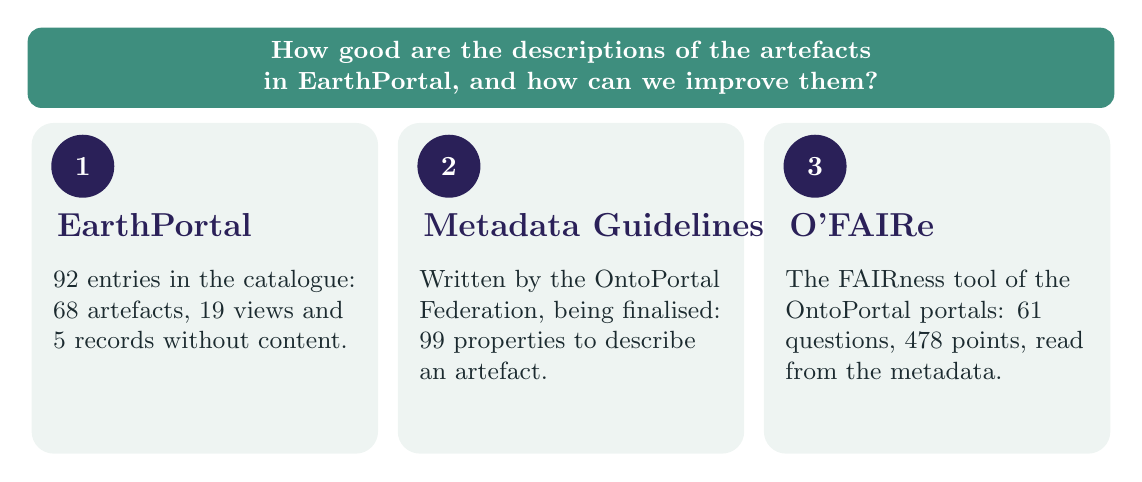
\begin{tikzpicture}
    \node[pill=epteal,minimum width=13.8cm,text width=13.4cm,font=\small\bfseries] at (0,2.2)
      {How good are the descriptions of the artefacts in EarthPortal, and how can we improve them?};
    \foreach \x/\n/\head/\body in {
      -4.65/1/EarthPortal/{92 entries in the catalogue: 68 artefacts, 19 views and 5 records without content.},
       0.00/2/{Metadata Guidelines}/{Written by the OntoPortal Federation, being finalised: 99 properties to describe an artefact.},
       4.65/3/O'FAIRe/{The FAIRness tool of the OntoPortal portals: 61 questions, 478 points, read from the metadata.}} {
      \node[card,minimum width=4.4cm,minimum height=4.2cm] at (\x,-0.6) {};
      \node[num=epnavy,minimum size=0.8cm,font=\normalsize\bfseries] at (\x-1.55,0.95) {\n};
      \node[text=epnavy,font=\large\bfseries,anchor=west] at (\x-2.0,0.2) {\head};
      \node[text=epink,font=\small,align=left,anchor=north west,text width=3.9cm] at (\x-2.05,-0.25) {\body};
    }
  \end{tikzpicture}
\end{frame}

% =====================================================================================================
% 3. What I was looking for
\begin{frame}{What I was looking for}
  \centering
  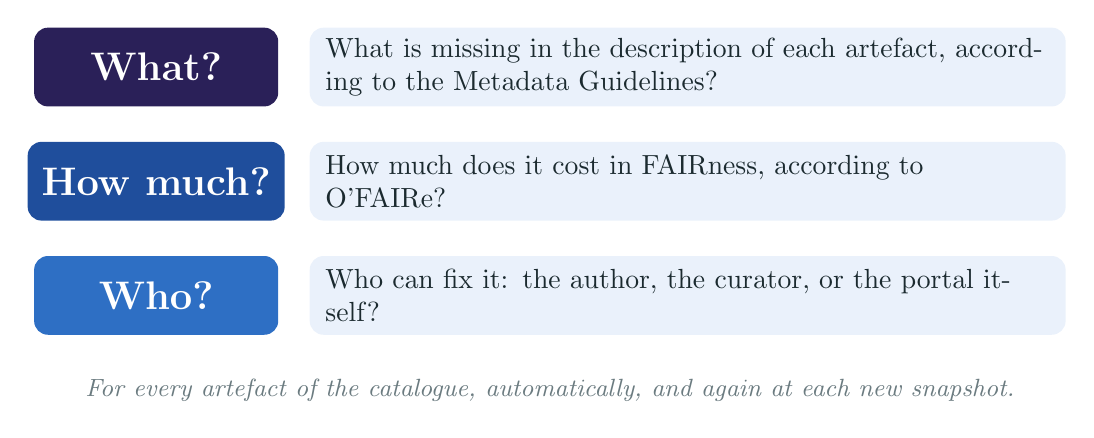
\begin{tikzpicture}
    \foreach \y/\c/\head/\body in {
       1.45/epnavy/What?/{What is missing in the description of each artefact, according to the Metadata Guidelines?},
       0.00/epblue/How much?/{How much does it cost in FAIRness, according to O'FAIRe?},
      -1.45/epmid/Who?/{Who can fix it: the author, the curator, or the portal itself?}} {
      \node[pill=\c,minimum width=3.1cm,minimum height=1.0cm,font=\Large\bfseries] at (-5.0,\y) {\head};
      \node[rounded corners=5pt,fill=epsky,text=epink,minimum width=9.6cm,minimum height=1.0cm,
            text width=9.2cm,align=left,font=\normalsize] at (1.75,\y) {\body};
    }
    \node[text=epgrey,font=\small\itshape] at (0,-2.65)
      {For every artefact of the catalogue, automatically, and again at each new snapshot.};
  \end{tikzpicture}
\end{frame}

% =====================================================================================================
% 4. Methodology
\begin{frame}{My methodology in four steps}
  \centering
  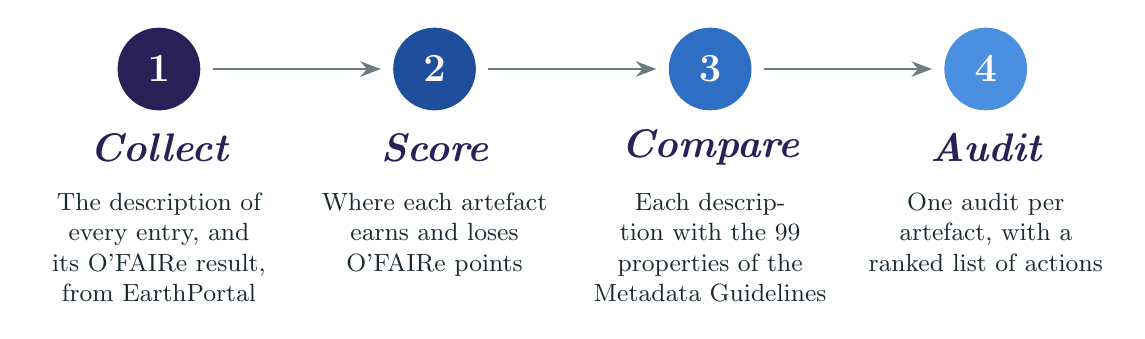
\begin{tikzpicture}
    \foreach \i/\x/\c/\head/\body in {
      1/-5.25/epnavy/Collect/{The description of every entry, and its O'FAIRe result, from EarthPortal},
      2/-1.75/epblue/Score/{Where each artefact earns and loses O'FAIRe points},
      3/1.75/epmid/Compare/{Each description with the 99 properties of the Metadata Guidelines},
      4/5.25/eplight/Audit/{One audit per artefact, with a ranked list of actions}} {
      \node[num=\c] (n\i) at (\x,1.4) {\i};
      \node[text=epnavy,font=\Large\bfseries\itshape] at (\x,0.4) {\head};
      \node[text=epink,font=\small,align=center,text width=3.1cm,anchor=north] at (\x,-0.05) {\body};
    }
    \foreach \a/\b in {1/2,2/3,3/4} \draw[arr] ($(n\a.east)+(0.15,0)$) -- ($(n\b.west)+(-0.15,0)$);
  \end{tikzpicture}\\[0.5cm]
  \raggedright\footnotesize
  \textbf{\textit{Open and reproducible:}}
  \href{https://github.com/EarthPortal/SA_Management}{\color{epblue}\underline{github.com/EarthPortal/SA\_Management}}~$\cdot$~DOI
  \href{https://doi.org/10.5281/zenodo.23417011}{\color{epblue}\underline{10.5281/zenodo.23417011}}
\end{frame}

% =====================================================================================================
% 5. From a missing property to an action (example: SWEET)
\begin{frame}{From a missing property to an action}
  \centering
  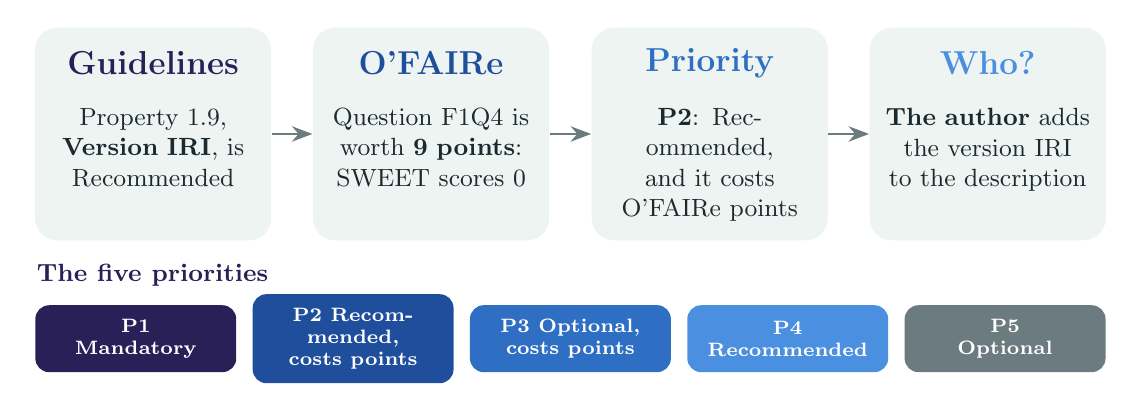
\begin{tikzpicture}
    \foreach \i/\x/\c/\head/\body in {
      1/-5.3/epnavy/{Guidelines}/{Property 1.9, \textbf{Version IRI}, is Recommended},
      2/-1.77/epblue/O'FAIRe/{Question F1Q4 is worth \textbf{9 points}: SWEET scores 0},
      3/1.77/epmid/Priority/{\textbf{P2}: Recommended, and it costs O'FAIRe points},
      4/5.3/eplight/Who?/{\textbf{The author} adds the version IRI to the description}} {
      \node[card,minimum width=3.0cm,minimum height=2.7cm] (c\i) at (\x,0.75) {};
      \node[text=\c,font=\large\bfseries] at (\x,1.65) {\head};
      \node[text=epink,font=\small,align=center,text width=2.75cm,anchor=north] at (\x,1.2) {\body};
    }
    \foreach \a/\b in {1/2,2/3,3/4} \draw[arr] (c\a.east) -- (c\b.west);
    % the five priorities
    \node[text=epnavy,font=\small\bfseries,anchor=west] at (-6.9,-1.05) {The five priorities};
    \foreach \x/\c/\t in {-5.52/epnavy/{P1\\Mandatory}, -2.76/epblue/{P2 Recommended,\\costs points},
                           0/epmid/{P3 Optional,\\costs points}, 2.76/eplight/{P4\\Recommended}, 5.52/epgrey/{P5\\Optional}}
      \node[pill=\c,font=\scriptsize\bfseries,minimum height=0.85cm,text width=2.2cm] at (\x,-1.85) {\t};
  \end{tikzpicture}\\[0.35cm]
  \raggedright\small\textit{The guidelines decide first; the O'FAIRe points then rank what is left.}
\end{frame}

% =====================================================================================================
% 6. Results on the catalogue
\begin{frame}{Results on the catalogue}
  \centering
  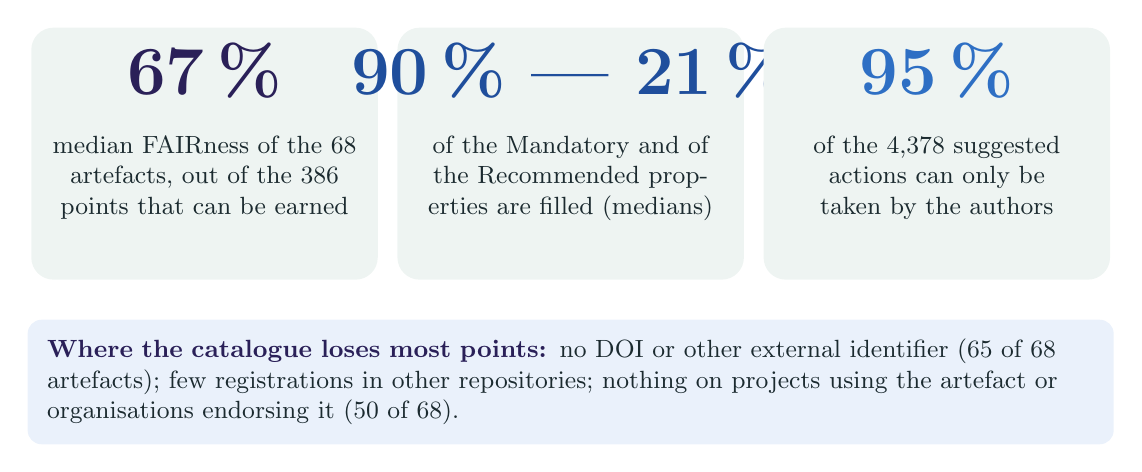
\begin{tikzpicture}
    \foreach \x/\c/\n/\body in {
      -4.65/epnavy/{67\,\%}/{median FAIRness of the 68 artefacts, out of the 386 points that can be earned},
       0.00/epblue/{90\,\% | 21\,\%}/{of the Mandatory and of the Recommended properties are filled (medians)},
       4.65/epmid/{95\,\%}/{of the 4,378 suggested actions can only be taken by the authors}} {
      \node[card,minimum width=4.4cm,minimum height=3.2cm] at (\x,0.8) {};
      \node at (\x,1.85) {\bignum{\c}{\n}};
      \node[text=epink,font=\small,align=center,text width=4.0cm,anchor=north] at (\x,1.15) {\body};
    }
    \node[rounded corners=5pt,fill=epsky,text=epink,minimum width=13.7cm,text width=13.3cm,align=left,
          font=\small,inner sep=7pt] at (0,-2.1)
      {\textbf{\color{epnavy}Where the catalogue loses most points:} no DOI or other external identifier
       (65 of 68 artefacts); few registrations in other repositories; nothing on projects using the
       artefact or organisations endorsing it (50 of 68).};
  \end{tikzpicture}\\[0.25cm]
  \raggedright\scriptsize\color{epgrey} Latest snapshot of the catalogue: 10 November 2026.
\end{frame}

% =====================================================================================================
% 7. Example: SWEET, part 1
\begin{frame}{One audit per artefact: SWEET}
  \begin{columns}[c]
    \begin{column}{0.64\textwidth}
      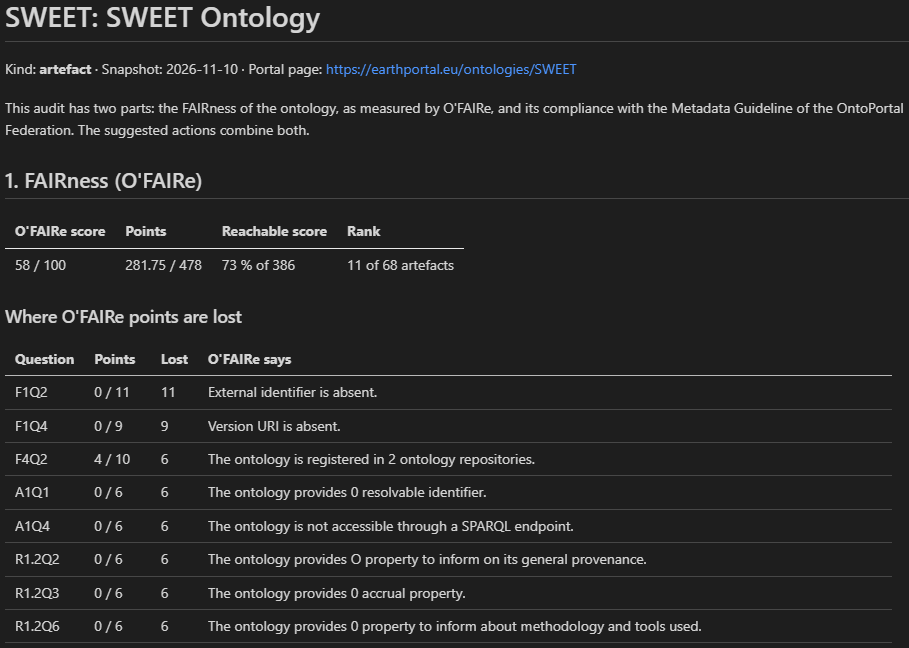
\includegraphics[width=0.8\linewidth]{Figures/slides_2026-11-13/SWEET_part1_crop.png}
    \end{column}
    \begin{column}{0.35\textwidth}
      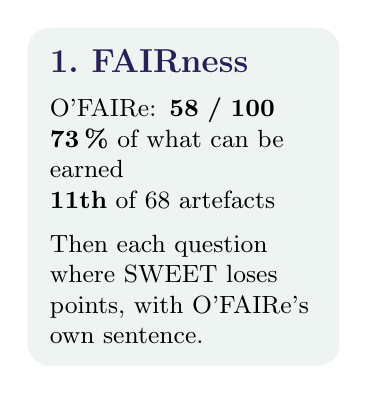
\begin{tikzpicture}
        \node[card,text width=3.4cm,align=left,inner sep=8pt,font=\small] {
          {\color{epnavy}\bfseries\large 1. FAIRness}\\[5pt]
          O'FAIRe: \textbf{58 / 100}\\
          \textbf{73\,\%} of what can be earned\\
          \textbf{11th} of 68 artefacts\\[5pt]
          Then each question where SWEET loses points, with O'FAIRe's own sentence.};
      \end{tikzpicture}
    \end{column}
  \end{columns}
  \vfill
  {\scriptsize\color{epgrey} \href{https://github.com/EarthPortal/SA_Management/blob/main/earthportal_sa_audit/audits/SWEET.md}{\texttt{audits/SWEET.md}} as shown by GitHub on 10 November 2026 (first rows).}
\end{frame}

% =====================================================================================================
% 8. Example: SWEET, part 2
\begin{frame}{One audit per artefact: SWEET}
  \begin{columns}[c]
    \begin{column}{0.64\textwidth}
      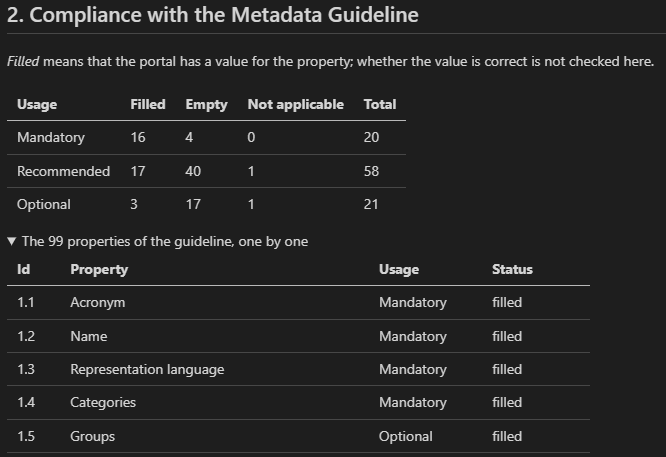
\includegraphics[width=0.5\linewidth]{Figures/slides_2026-11-13/SWEET_part2_crop.png}\\[3pt]
      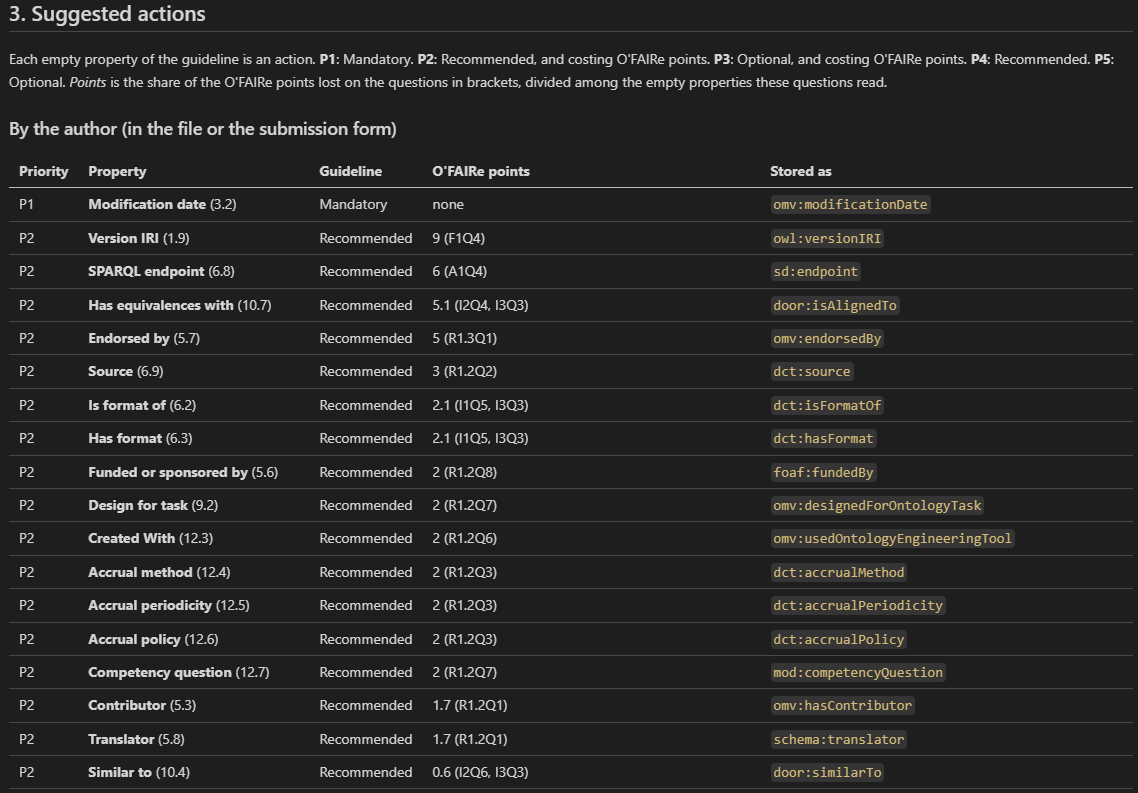
\includegraphics[width=0.6\linewidth]{Figures/slides_2026-11-13/SWEET_part3_crop.png}
    \end{column}
    \begin{column}{0.35\textwidth}
      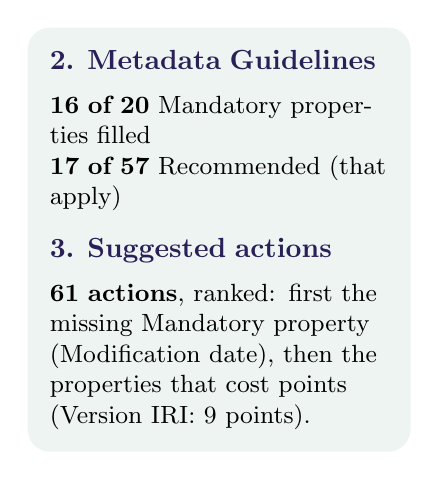
\begin{tikzpicture}
        \node[card,text width=4.3cm,align=left,inner sep=8pt,font=\small] {
          {\color{epnavy}\bfseries\normalsize 2. Metadata Guidelines}\\[5pt]
          \textbf{16 of 20} Mandatory properties filled\\
          \textbf{17 of 57} Recommended (that apply)\\[8pt]
          {\color{epnavy}\bfseries\normalsize 3. Suggested actions}\\[5pt]
          \textbf{61 actions}, ranked: first the missing Mandatory property (Modification date), then
          the properties that cost points (Version IRI: 9 points).};
      \end{tikzpicture}
    \end{column}
  \end{columns}
\end{frame}

% =====================================================================================================
% 9. What I propose
\begin{frame}{What I propose}
  \centering
  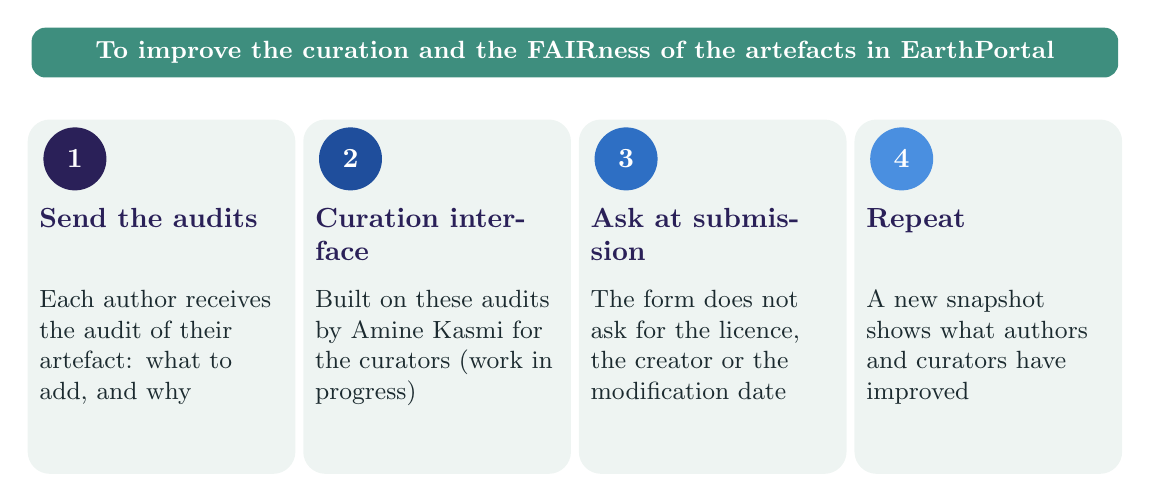
\begin{tikzpicture}
    \node[pill=epteal,minimum width=13.8cm,text width=13.4cm,font=\small\bfseries] at (0,2.75)
      {To improve the curation and the FAIRness of the artefacts in EarthPortal};
    \foreach \i/\x/\c/\head/\body in {
      1/-5.25/epnavy/{Send the audits}/{Each author receives the audit of their artefact: what to add, and why},
      2/-1.75/epblue/{Curation interface}/{Built on these audits by Amine Kasmi for the curators (work in progress)},
      3/1.75/epmid/{Ask at submission}/{The form does not ask for the licence, the creator or the modification date},
      4/5.25/eplight/{Repeat}/{A new snapshot shows what authors and curators have improved}} {
      \node[card,minimum width=3.4cm,minimum height=4.5cm] at (\x,-0.35) {};
      \node[num=\c,minimum size=0.8cm,font=\normalsize\bfseries] at (\x-1.1,1.4) {\i};
      \node[text=epnavy,font=\normalsize\bfseries,align=left,text width=3.1cm,anchor=north] at (\x,0.9) {\head};
      \node[text=epink,font=\small,align=left,text width=3.1cm,anchor=north] at (\x,-0.15) {\body};
    }
  \end{tikzpicture}
\end{frame}

% =====================================================================================================
% 10. Thank you, with two QR codes: the software (concept DOI, always the latest release) and these
%     slides (version DOI 10.5281/zenodo.24132003, reserved on Zenodo on 11 November 2026)
{\darkbackground
\begin{frame}[plain]
  \begin{tikzpicture}[remember picture,overlay]
    \node[text=white,font=\fontsize{26}{30}\selectfont\bfseries] at ($(current page.center)+(-3.7cm,1.35cm)$) {Thank you};
    \node[text=white,font=\normalsize,align=center] at ($(current page.center)+(-3.7cm,0.45cm)$)
      {Vielen Dank $\cdot$ Merci beaucoup\\[2pt]Grazie mille};
    \node[text=white,font=\footnotesize\itshape,align=center] at ($(current page.center)+(-3.7cm,-0.75cm)$)
      {\href{https://github.com/EarthPortal/SA_Management}{github.com/EarthPortal/SA\_Management}};
    \foreach \x/\file/\head/\doi in {
      1.75/QR_software_concept_DOI/Software/{10.5281/zenodo.23417011},
      5.45/QR_slides_TIB_version_DOI/{These slides}/{10.5281/zenodo.24132003}} {
      \node[fill=white,rounded corners=6pt,inner sep=5pt] at ($(current page.center)+(\x cm,0.75cm)$)
        {\includegraphics[width=2.2cm]{Figures/slides_2026-11-13/\file.png}};
      \node[text=white,font=\small\bfseries] at ($(current page.center)+(\x cm,-0.85cm)$) {\head};
      \node[text=white!85,font=\scriptsize] at ($(current page.center)+(\x cm,-1.25cm)$) {\doi};
    }
  \end{tikzpicture}
\end{frame}
}

\end{document}
